\problemname{Security Zone}
The manager of a large security company has to build a new surveillance system for different sites.
A site consists of $N$ objects where each object has its own security circle.
At the border of the surveillance system a high voltage fence has to be installed.
The security zone inside of the fence has to be connected.
Furthermore, all objects and their security circles should be inside the security zone.
The security circles of different objects will never overlap or touch.
Now the manager needs your help.
He asks you for the minimal needed fence length.

\begin{figure}[h]
	\centering
	\hfill
	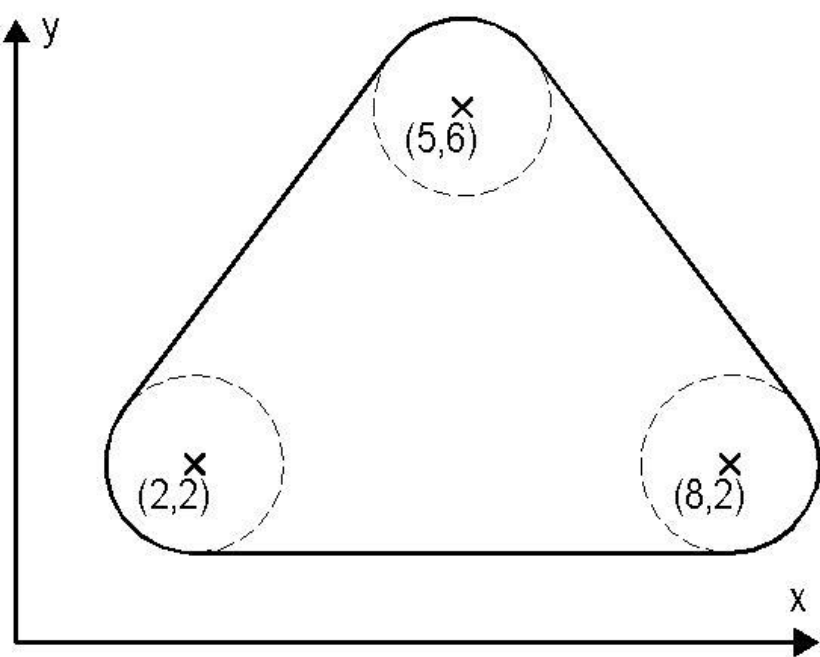
\includegraphics[width=0.3\textwidth]{image1}\hfill
	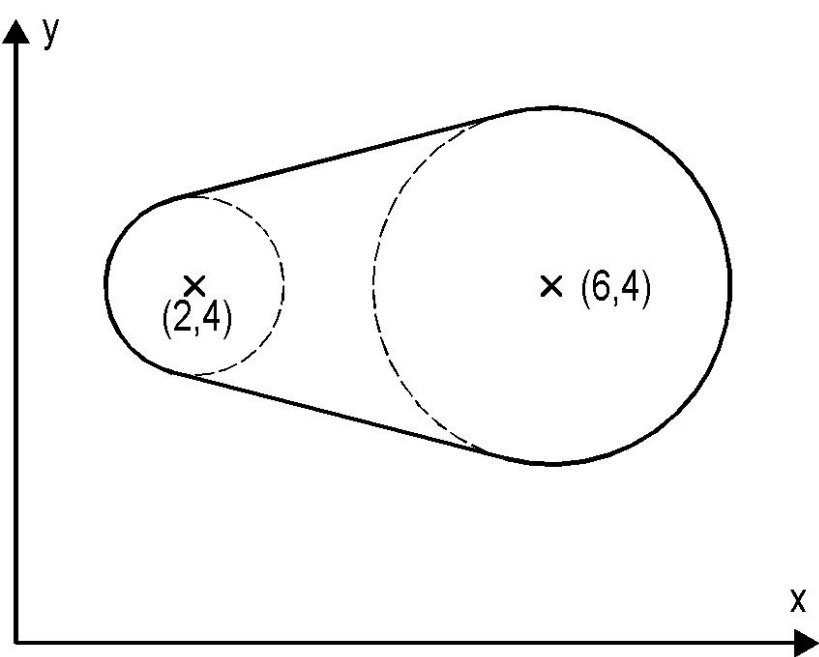
\includegraphics[width=0.3\textwidth]{image2}\hfill
	\mbox{}
	\caption{Illustration of first and second sample input.}
\end{figure}

\begin{Input}
    The first line of the input gives the number of test cases $C$ ($0 \leq C \leq 100$).
    The first line of each such test case holds the integer $N$:
    the number of objects in the current site ($0 < N \leq 25$).
    Each of the following $N$ lines holds three integers $x_i$, $y_i$, and $r_i$ that describe an object.
    The coordinates of the i-th object and the radius for the needed security circle for this object.
    ($|x_i |, |y_i | \leq 100$, $0 < r_i \leq 100$)
    (The center of the security circle around an object is the position of the object itself.)
\end{Input}

\begin{Output}
    For each test case print one line containing the minimal fence length for this case.
    Your output should have an absolute or relative error of at most $10^{-7}$.
\end{Output}
